\chapter{Equipment}
\label{ch:equipment}

Fantasy roleplaying games can be thought of as a form of cooperative improvised theatre. You could think of the players as the actors and the Gamemaster as the director and production team providing the stage and scenery, a huge big budget supporting cast and every prop that the actors could possibly need. This chapter deals with the props, the equipment that the player characters will be using.

\section{In-game Economics}
These rules do not provide details for trading and fantasy world economics. Although dry economic markets are unlikely to feature heavily in adventure stories, the exploits of daring and wily merchant adventurers are. %The following section outlines how to approach such stories using Fantasy Crux.

%\subsection{Merchant based Games}
%Some players will feel inclined to create colourful and flamboyant Merchant characters and weave stories around their trade missions to far off unexplored countries creating drama and tension on their trade negotiations and deals. This is great and is to be encouraged. Opposed Trade tests can be used to handle the outcome of such action where it is less than clear cut, and the ebb and flow of the character’s finances acts as an indicator of success (see the Trade skill description on page~\pageref{ssec:trade}). The more martially and magically inclined characters can provide support and have their moments in the spotlight too on these mercantile adventures, taking on the villains hired by their rivals in commerce. If you are in need of inspiration then you only have to look to the real life historical adventures of Marco Polo.

%Merchant characters also make great information gatherers, since they tend to have good social skills. Often this goes on under the cover of trading in the market, gathering gossip from the locals, or sorting out a new trade deal with a noble family, which is a legitimate way of finding information about a noble.

\subsection{Availability of Goods}
The equipment lists serve as ‘game tools’ to allow players to quickly and easily buy equipment for their characters. The range of goods listed at the quoted prices is only going to be available in a large metropolis with organised markets and districts given over to shops and mercantile activity. 

In less prosperous cities and towns there is a smaller range available, sometimes at higher costs. In rural areas, only local produce and a small amount of locally crafted goods can be bought at a reasonable price. There might be oddities to this model and these can lead to further adventure. 

\begin{rpg-examplebox}
A village without an armourer has a large cache of old armour and weapons for sale at a good price. This is because a local monster living in a nearby cave has been ambushing and killing adventurers for years and then trading their equipment to the villagers. In turn, the villagers oblige by sending a steady stream of fresh and inexperienced adventurers, such as the recently arrived player characters, to its lair.
\end{rpg-examplebox}

\subsection{Barter}
Coins are the main exchange method for the landed nobility and rich merchants. Barter is the main method of exchanging goods for people outside of the main urban areas. In such transactions successful Opposed Test using the Trade of the buyer versus the Trade of the seller are needed for the buyer to get the best deal.


\subsection{Consequences}
The main thing to remember is that with any item of equipment there are consequences in their use as well as benefits. The most obvious consequence is encumbrance. A heavily armoured and equipped character will be slowed, unable to use skills as effectively and will become fatigued more easily.

A less obvious effect is that an obviously well equipped character becomes a target for both minor and major theft. From the opportunistic thief who desires the PC’s new sword to the more organised bandit group who targets the party because they believe that they have a stash of treasure back at their base because of all the flashy new equipment they are wearing.

There might also be social consequences. In civilised towns and cities, prominent displays of arms and armour may unsettle and upset the locals and bring about the unwanted attention of the Watch who want to make sure that the characters are not violent troublemakers. In some more draconian fantasy lands there may even be laws and social codes that dictate what arms and armour a citizen may own and in what situations they may carry it. 

\subsection{Currency}
Coins are usually created in mints tightly controlled by the local nobility, appointed by the local ruler, whose head appears on one side of the coin. Other sources of coin are usually the treasure troves of monsters, whose assets are brought into the economy by enterprising adventurers.

Currency can be based upon whatever is valued by the culture using it. Being a fantasy game, many variant systems of currency can be created. For example, a system that uses the teeth of slain dragons or magical gemstones enchanted with minor magic that is useful in everyday life can be used as an exchange mechanism.

For ease of use here’s a simple coin based currency that will be used throughout the rest of this book to give value to an item.

\vspace{1em}

\begin{rpg-table}[|X|]
	\hline
%        5 Lead Bits (LB) = 1 Copper Penny (CP)\\
%	10 Copper Pennies (CP) = 1 Silver Piece (SP)\\
%	20 Silver Pieces (SP) = 1 Gold Ducat (GD)\\
	10 Copper Pieces (CP) = 1 Silver Piece (SP)\\
	10 Silver Pieces (SP) = 1 Gold Piece (GP)\\
	\hline
\end{rpg-table}

\section{The Equipment Lists}
The rest of this chapter is given over to equipment lists. These lists provide the cost of the item and detail any game effects. They also give an Encumbrance value (ENC) for the item in question. This is a value which rates both the weight and how physically unwieldy an item is. This is for the Encumbrance rules given on page~\pageref{ssec:encumbrance}.

\begin{figure}[h]
\begin{center}
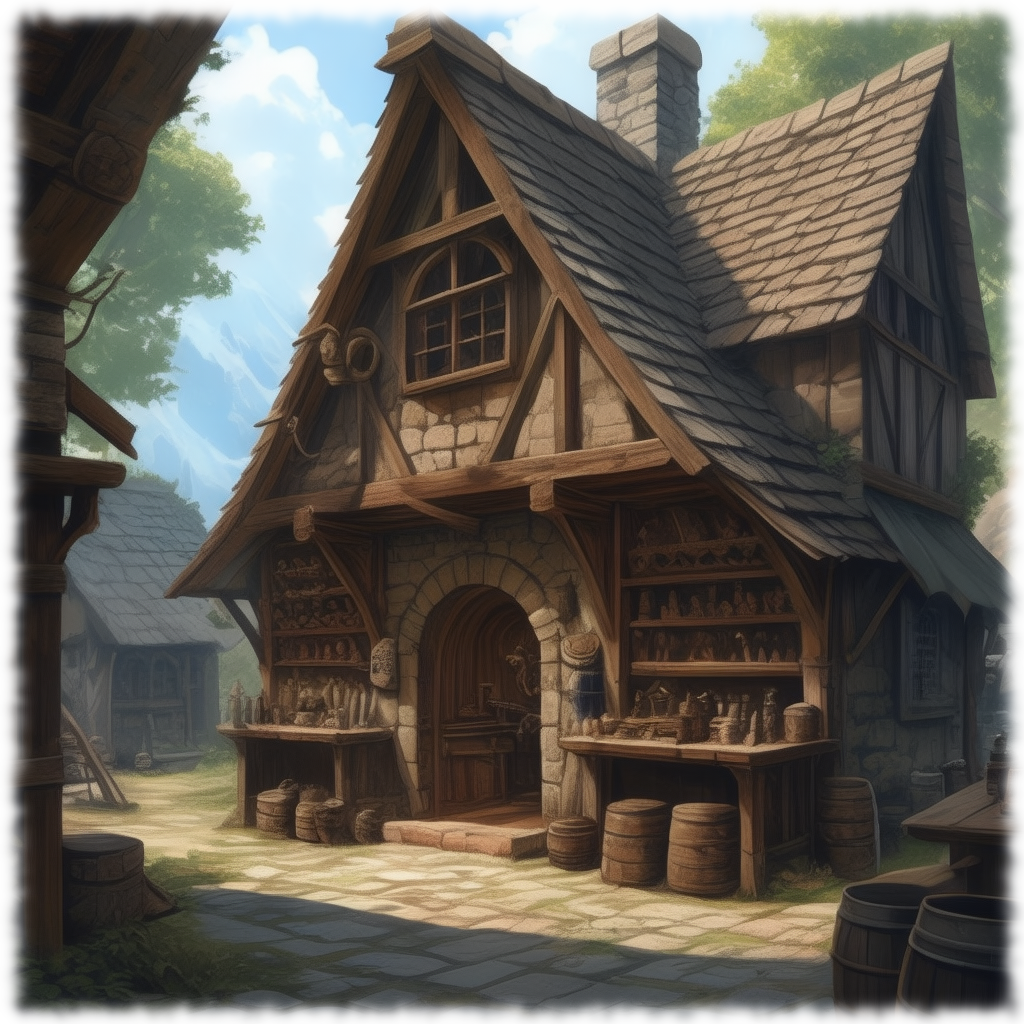
\includegraphics[scale=0.24]{img/ai-images/shop.png}
\end{center}
\end{figure}

\section{Close Combat Weapons}
All Close Combat weapons use the Close Combat skill. Each close combat weapon is characterised by the following qualities: 

\begin{description}
	\item[Type:] This shows how the weapon is wielded and other special rules (see Close Combat Weapon Types on page~\pageref{sssec:close-combat-weapon-types}).
	\item[Damage Dice:] The damage the weapon deals on a successful attack. 
	\item[STR/DEX:] The minimum STR and DEX scores needed to easily wield this weapon. If either of the Characteristics are below these minimums, a –20\% maximum penalty is applied to a character’s skill when attacking and parrying with this weapon. 
	\item[ENC:] The weapon’s Encumbrance. The weight and bulk of the weapon. 
	\item[Size:] Weapons are rated in the following size categories: Light, Medium, Heavy and Huge. Weapons need to be of the same category or larger to block all damage. If the defending weapon is one category less they block half damage. If two categories less they cannot block the damage.
	\item[Cost:] The cost in silver pieces to purchase this weapon. 
\end{description}

\begin{table*}[h]
\begin{center}
\caption{Close Combat Weapons}
\label{tab:close-combat-weapons}
\begin{rpg-table}[|X|c|c|c|c|c|c|]
	\hline
	\textbf{Weapon} & \textbf{Type} & \textbf{Damage Dice} & \textbf{STR/DEX} & \textbf{ENC} & \textbf{Size} & \textbf{Cost}\\
	\hline
	%\multicolumn{7}{|l|}{\textbf{Swords and Knives}}\\
	%\hline
	Arming Sword    & 1H             & 1D8   &  9/9  & 2 & Medium & 150 SP\\
	Ball and Chain  & 1H             & 1D8   &  9/9  & 2 & Medium & 120 SP\\
	Battleaxe       & 1H             & 1D8   &  9/9  & 2 & Medium & 120 SP\\
	Club            & Flex           & 1D6   &  5/9  & 1 & Light  & 20 SP\\
	Dagger          & 1H/Range       & 1D4+1  &  -/-  & - & Light  & 20 SP\\
	Great Axe       & 2H             & 2D8   & 13/5  & 4 & Heavy  & 200 SP\\
	Great Hammer    & 2H             & 2D8   & 13/5  & 4 & Heavy  & 200 SP\\
	Greatsword      & 2H             & 2D8   & 13/9  & 4 & Heavy  & 300 SP\\
	Hatchet         & 1H/Range       & 1D6   &  5/9  & 1 & Light  & 20 SP\\
	Lance           & Flex/Set       & 1D10  & 11/9  & 3 & Heavy  & 150 SP\\
	Longspear       & 2H/Set         & 1D8+1 &  9/5  & 2 & Medium & 30 SP\\
	Longsword       & Flex           & 1D8   & 13/11 & 2 & Medium & 250 SP\\
	Mace            & Flex           & 1D8   &  9/9  & 2 & Medium & 120 SP\\
	Military Flail  & 2H             & 2D8   & 13/5  & 4 & Heavy  & 200 SP\\
	Polearm         & 2H/Set         & 1D8   &  9/9  & 3 & Heavy  & 200 SP\\
	Quarterstaff    & 2H             & 1D8   &  5/9  & 2 & Medium & 20 SP\\
	Scimitar        & 1H             & 1D8   &  9/9  & 2 & Medium & 150 SP\\
	Shield (small)  & -              & 1D4   &  -/-  & 1 & Medium & 50 SP\\
	Shield (medium) & -              & 1D6   &  9/-  & 2 & Heavy  & 150 SP\\
	Shield (large)  & -              & 1D6   & 13/-  & 3 & Huge   & 300 SP\\
	Shortspear      & Flex/Set/Range & 1D6   &  5/5  & 2 & Medium & 20 SP\\
	Shortsword      & 1H             & 1D6   &  5/5  & 1 & Medium & 100 SP\\
	Unarmed         & -              & 1D3   &  -/-  & - & -      & -\\
	War Hammer      & 1H             & 1D8   &  9/9  & 2 & Medium & 120 SP\\
	\hline
\end{rpg-table}
\end{center}
\end{table*}

\subsubsection{Close Combat Weapon Types}
\label{sssec:close-combat-weapon-types}
\begin{description}
	\item[1H:] This weapon must be used one-handed.
	\item[2H:] This weapon must be used two-handed.
	\item[Flex:] This weapon can be used two-handed.  When used in two hands, it gains +2 damage and can be used by someone with a STR 2 less than that listed.
	\item[Set:] This weapon may be set against a charge. The wielder must state, however, at the start of combat how it is being wielded and must take a Change Stance action to alter its usage.
	\item[Range:] This weapon suffers no penalty when thrown. 
	%\item[LS:] This weapon may be used as a Longspear. If used as a Longspear it may be set against charges. The wielder must state, however, at the start of combat how it is being wielded and must take a Change Stance action to alter its usage. 
\end{description}

Note that improvised and primitive weapons: such as a stone hatchet, stone spear or a convenient log picked up and used as a club, do the same damage as the base weapon -1.

\section{Ranged Weapons}
Each ranged weapon is characterised by the following qualities:
\begin{description}
	\item[Type:] This shows how the weapon is wielded and other special rules (see Ranged Combat Weapon Types on page~\pageref{sssec:ranged-combat-weapon-types}).
	\item[Damage Dice:] The damage the weapon deals on a successful attack. 
	\item[Range:] This is the effective range of the weapon. A target within the weapon’s range may be attacked without penalty. A target within double the weapon’s range may be attacked, but the attacker’s effective Weapon skill is halved (before other modifiers are applied). Attacks against targets beyond double the weapon’s range automatically fail.
	\item[STR/DEX:] The minimum STR and DEX scores required to easily wield this weapon. If either of the Characteristics are below these minimums, a maximum –20\% penalty is applied to a character’s skill when attacking and parrying with this weapon.
	\item[ENC:] The weapon’s Encumbrance. The weight and bulk of the weapon. 
	\item[Cost:] The cost in silver pieces to purchase this weapon.
\end{description}


\begin{table*}[h]
\begin{center}
\caption{Ranged Combat Weapons}
\label{tab:ranged-combat-weapons}
\begin{rpg-table}[|X|c|c|c|c|c|c|]
	\hline
	\textbf{Weapon} & \textbf{Type} & \textbf{Damage Dice} & \textbf{Range} & \textbf{STR/DEX} & \textbf{ENC} & \textbf{Cost}\\
	\hline
	Dagger            & Close/Thrown   & 1D4+1 & STR x m  & -/9  & -  & 30 SP\\
	Dart              & Thrown         & 1D3   & STR x m  & -/9  & -  & 15 SP\\
	Crossbow (Heavy)  & 2H             & 2D6   & 150m     & 9/9  & 2  & 350 SP\\
	Crossbow (Light)  & 2H             & 1D8   & 125m     & 5/9  & 1  & 150 SP\\
	Hatchet           & Close/Thrown   & 1D6   & STR x m  & -/9  & 1  & 25 SP\\
	Improvised (Rock) & Thrown         & 1d4   & STR x m  & 5/5  & 1  & -\\
	Javelin           & Thrown         & 1d6   & STR x 2m & 5/9  & 1  & 20 SP\\
	Longbow           & 2H             & 1d10  & 150m     & 13/9 & 1  & 150 SP\\
	Shortbow          & 2H             & 1d8   & 75m      & 9/9  & 1  & 75 SP\\
	Shortspear        & Close/Thrown   & 1d6   & STR x 2m & 5/9  & 2  & 20 SP\\
	Sling             & 1H             & 1d6   & 50m      & -/9  & -  & 5 SP\\
	Whip              & Close          & 1d3   & 5m       & -/9  & -  & 50 SP\\
	\hline
\end{rpg-table}
\end{center}
\end{table*}

\subsubsection{Ranged Combat Weapon Types}
\label{sssec:ranged-combat-weapon-types}
\begin{description}
	\item[1H:] This weapon must be used one-handed.
	\item[2H:] This weapon must be used two-handed. A small shield (e.g. buckler) can be strapped to the forearm but cannot be used whilst wielding or shooting this weapon.
	\item[Close:] This weapon suffers no penalty when used in Close Combat.
	\item[Thrown:] A character can use his/her damage modifier with this weapon.
	\item[Range:] This weapon suffers no penalty at this distance. 
\end{description}


\subsubsection{Using Ranged Weapons in Close Combat}
If used in close combat, a ranged weapon is treated as an improvised weapon, doing damage equal to its closest hand-to-hand equivalent if that is less than its ranged weapon damage.


\begin{table}
\begin{center}
\caption{Ranged Weapon Ammunition}
\label{tab:ranged-weapon-ammunition}
\begin{rpg-table}[|X|c|c|]
	\hline
	\textbf{Ammunition} & \textbf{ENC} & \textbf{Cost}\\
	\hline
	Arrows (10)         & - & 1 SP\\
	Blowgun darts (10)  & - & 2 SP\\
	Crossbow bolts (10) & - & 2 SP\\
	Sling bullets (10)  & - & 5 CP\\
	\hline
\end{rpg-table}
\end{center}
\end{table}


\begin{figure}[h]
\begin{center}
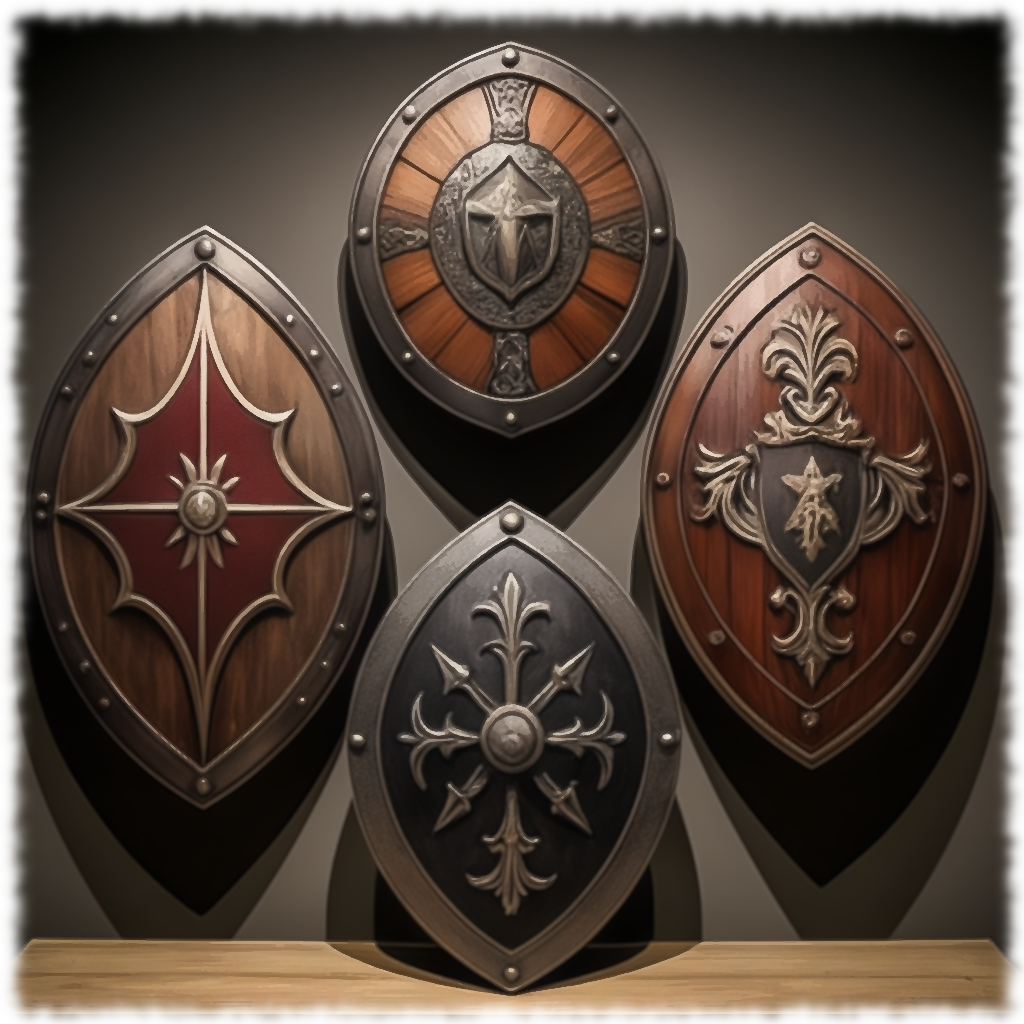
\includegraphics[scale=0.24]{img/ai-images/shields.png}
\end{center}
\end{figure}

\section{Armour}
Each piece of armour is characterised by the following qualities: 
\begin{description}
	\item[AP:] How many armour points this type of armour provides. In case you need variable armour values use the value in parenthesis (usefull, if the averages give no chance of damaging).
	\item[ENC:] The armour’s Encumbrance. The weight and bulk of the armour. The character's base Combat Order is reduced by the ENC value of the armour.
	\item[Cost:] The cost in silver pieces to purchase this armour. 
\end{description}

\begin{table}
\begin{center}
\caption{Armours}
\label{tab:armors}
\begin{rpg-table}[|X|c|c|c|]
	\hline
	\textbf{Armour} & \textbf{AP} & \textbf{ENC} & \textbf{Cost}\\
	\hline
	Leather      & 2 (1D3)   & 3 & 500 SP\\
	Ringmail     & 3 (1D4)   & 4 & 1000 SP\\
	Scalemail    & 4 (1D6)   & 6 & 1500 SP\\
	Chainmail    & 5 (2D4)   & 7 & 3000 SP\\
	Platemail    & 6 (2D6)   & 9 & 9000 SP\\
	\hline
\end{rpg-table}
\end{center}
\end{table}


\begin{figure}[h]
\begin{center}
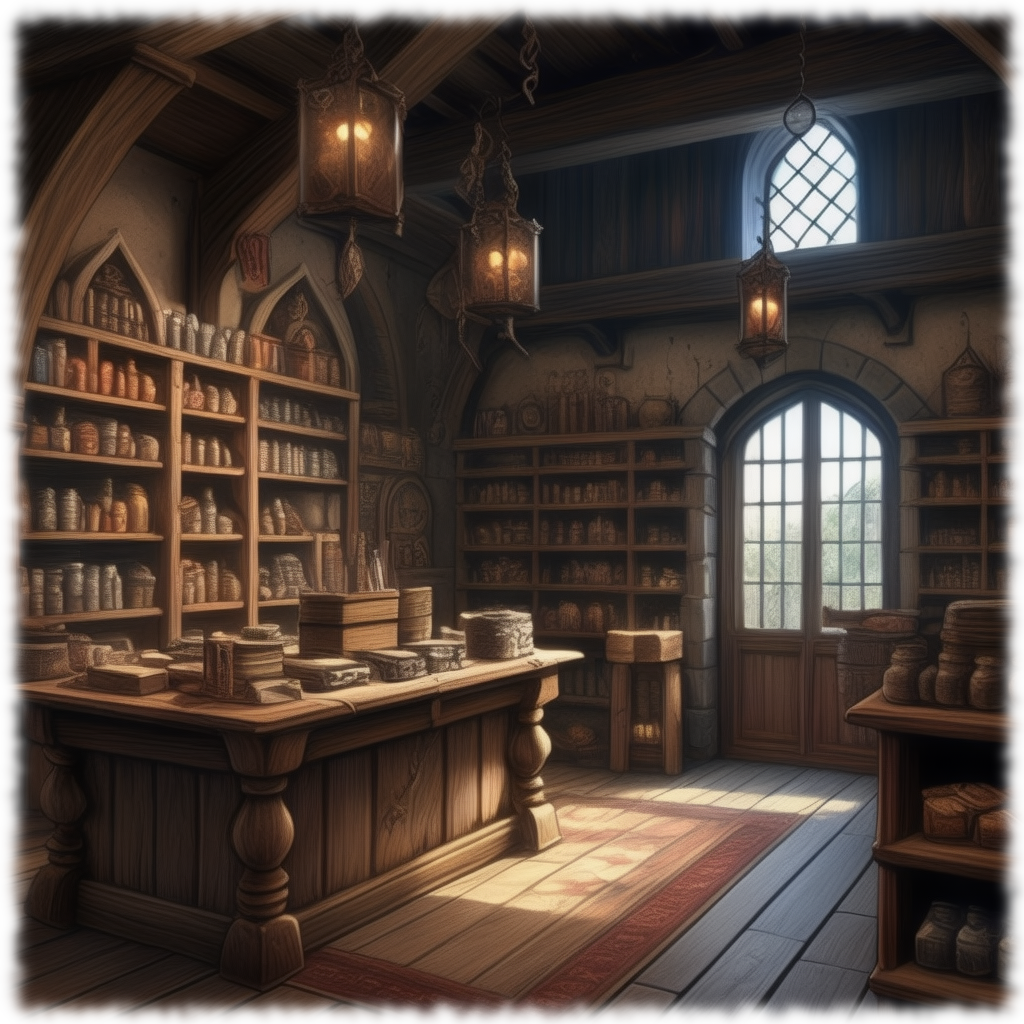
\includegraphics[scale=0.24]{img/ai-images/shop-interior.png}
\end{center}
\end{figure}

\subsubsection{Armour Descriptions}
\begin{description}
	\item[Leather:] Either padded leather or boiled and stiffened leather or linen armour.
	\item[Ringmail:] Metal rings sown onto a padded leather suit.
	\item[Scalemail:] Metal scales sown onto a padded leather suit.
	\item[Chainmail:] Links of chain made into a suit.
	\item[Platemail:] Steel plates that cover the body, over a chain mail backing.
\end{description}


\subsubsection{Effects of SIZ on Armour}
Armour made for a character of SIZ 1 to 5 will have its cost and ENC halved from that shown on table~\ref{tab:armors}. Characters of SIZ 21 or higher will double the cost and ENC for armour made for them.

Also note that:
\begin{rpg-list}
	\item Characters may try using plate armour not designed for them but the ENC will be doubled. 
	\item Characters may not wear more than one type of armour, i.e. layer armour, to get increased Armour Points. 
\end{rpg-list}



\section{General Items}
\begin{table}[!h]
\begin{center}
\caption{General Items}
\label{tab:general-items}
\begin{rpg-table}[|X|Y|Y|]
	\hline
	\textbf{Item} & \textbf{ENC} & \textbf{Cost}\\
	\hline
	Backpack                  & 1 & 5 SP\\
	Bedroll                   & 1 & 1 SP\\
	Block \& Tackle           & 1 & 15 SP\\
	Bottle, glass             & - & 2 SP\\
	Candle, 1 hour            & - & 1 CP\\
	Chain, 2 metres           & 2 & 40 SP\\
	Climbing Kit              & 1 & 25 SP\\
	Craft Tools               & 2 & 75 SP\\
	Crowbar                   & 1 & 25 SP\\
	Healing Kit               & - & 25 SP\\
	Fish Hook                 & - & 1 CP\\%2 LB\\
	Fishing Kit               & 1 & 15 SP\\
	Flint \& Tinder           & - & 5 CP\\
	Grappling Hook            & - & 5 SP\\
	Hammer                    & - & 1 SP\\
	Ladder, 3 metres          & 4 & 2 SP\\
	Lantern                   & 1 & 10 SP\\
	Lock Picks                & - & 75 SP\\
	Mining Pick               & 1 & 35 SP\\
	Musical Instrument        & 2 & 70 SP\\
	Oil, Flask                & 1 & 1 SP\\
	Papyrus, Sheet            & - & 1 SP\\
	Quiver                    & - & 2 SP\\
	Rope, 10 metres           & 2 & 10 SP\\
	Sack, Large               & 1 & 5 CP\\
	Sack, Small               & - & 2 CP\\
	Scythe                    & 2 & 30 SP\\
	Slingbag                  & 1 & 5 CP\\
	Spade                     & 1 & 25 SP\\
	Torch                     & - & 4 CP\\
	Waterskin                 & 1 & 5 CP\\
	Writing Kit               & 1 & 45 SP\\
	\hline
\end{rpg-table}
\end{center}
\end{table}



\begin{description}
	\item[Backpack:] It can hold 20 ENC of equipment. 
	\item[Block \& Tackle:] Adds +20\% to Mechanisms tests to make or disarm large traps and makes Engineering tests possible in some circumstances. It requires at least 10m of rope to function. 
	\item[Candle, 1 Hour:]  A candle illuminates a one metre radius. Any wind stronger than a slight breeze will extinguish a candle. 
	\item[Climbing Kit:]  A climbing kit provides a bonus of +20\% to any Athletics skill tests made to climb. 
	\item[Crowbar:] Adds +20\% to brute force Athletics tests. If used as a weapon, it is considered a club (wielded with a –20\% penalty). 
\end{description}


\begin{description}
	\item[Healing Kit:] A healing kit is good for five uses (whether the skill test succeeds or fails). 
	\item[Fish Hook:] This item allows a character to use his Natural Lore skill to catch a fish without suffering a penalty on the test. 
\end{description}



\begin{description}
	\item[Fishing Kit:] The fishing kit grants a character a +20\% bonus to his Natural Lore test to catch fish. 
	\item[Flint \& Tinder:] A character with flint and tinder can build a fire in one minute under normal conditions without having to roll his Natural Lore skill. 
	\item[Grappling Hook:] It will support the weight of 50 ENC or 50 SIZ, or any combination thereof. 
	\item[Hammer:] If used as a weapon, it is treated as a club (wielded with a –20\% penalty). Hammers may be used on inanimate objects without being destroyed. 
	\item[Lantern:] A lantern provides clear illumination out to a three metre radius. It will burn for two hours on a flask of oil. 
	\item[Lock Picks:] Adds +20\% to Mechanisms tests to unlock a locking device. 
	\item[Mining Pick:] If used as a weapon, it is considered a club (wielded with a –20\% penalty). Mining picks may be used on inanimate objects without being destroyed. 
	\item[Oil, Flask:] A flask of oil is enough to fuel a lantern for two hours or, if broken on the ground and ignited, enough to sustain a small fire for one minute. 
	\item[Quiver:] Quivers can hold up to 30 arrows or crossbow bolts. 
	\item[Rope, 10 Metres:] A standard rope can support the weight of 50 ENC or 50 SIZ, or any combination thereof. 
	\item[Sack, Large:] Able to hold 10 ENC of equipment. 
	\item[Sack, Small:] A small sack can hold 5 ENC of equipment. 
	\item[Scythe:] If used as a weapon, it is considered a polearm (wielded with a –20\% penalty). 
	\item[Slingbag:] It can carry 15 ENC of equipment. 
	\item[Spade:] If used as a weapon, it is considered a club (wielded with a –20\% penalty). 
	\item[Torch, 1 Hour:] It will burn for one hour. A torch illuminates a three metre radius. If used as a weapon, it is considered a club (wielded with a –20\% penalty), except that it does not inflict normal damage – instead, it inflicts 1D4 fire damage and a fumble or critical hit will also extinguish the brand. 
	\item[Waterskin:] A waterskin can hold enough water to sustain an adventurer for two days.
\end{description}

\begin{figure}[!h]
\begin{center}
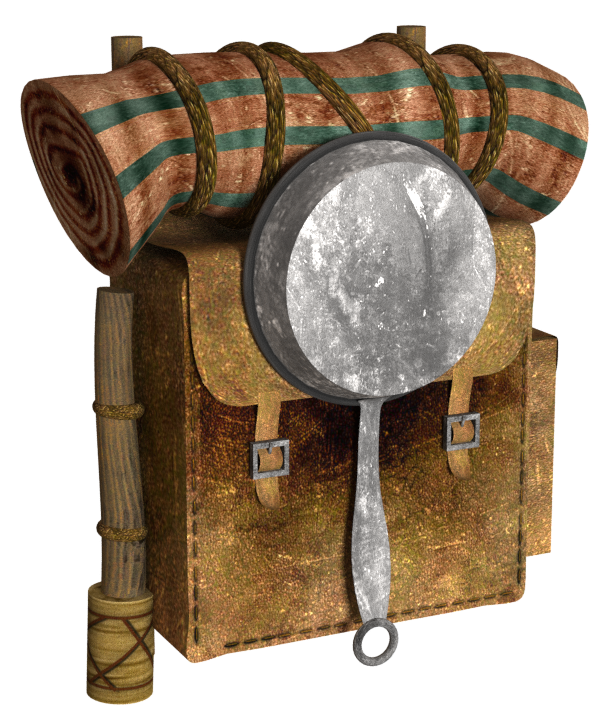
\includegraphics[scale=0.2]{img/Backpack.png}
\end{center}
\end{figure}

\pagebreak

\section{Transportation}
Some example prices for trading animals as well as transportation services can be found in the following table.

\begin{table}[H]
\begin{center}
\caption{Animals and Transportation}
\label{tab:animals-and-transportation}
\begin{rpg-table}[|X|Y|]
	\hline
	\textbf{Animal} & \textbf{Cost}\\
	\hline
	Bison                  & 200 SP\\
	Bull                   & 250 SP\\
	Cart                   & 75 SP\\
	Cat                    & 2 SP\\
	Chariot                & 600 SP\\
	Cow                    & 150 SP\\
	Dog, Domestic          & 2 SP\\
	Dog, Hunting           & 25 SP\\
	Fowl                   & 1 SP\\
	Goat                   & 50 SP\\
	Hawk                   & 400 SP\\
	Horse, Draft           & 400 SP\\
	Horse, Riding          & 350 SP\\
	Horse, Combat Trained  & 500 SP\\
	Mule                   & 125 SP\\
	Ox                     & 200 SP\\
	Pig                    & 50 SP\\
	Saddle and Bridle      & 75 SP\\
	Sheep                  & 30 SP\\
	Travel (by Post-Horse) & 2 SP per kilometre\\
	Travel (by Ship)       & 1 SP per kilometre\\
	Travel (by Wagon)      & 5 SP per kilometre\\
	Wagon                  & 300 SP\\
	\hline
\end{rpg-table}
\end{center}
\end{table}


\begin{figure}
\begin{center}
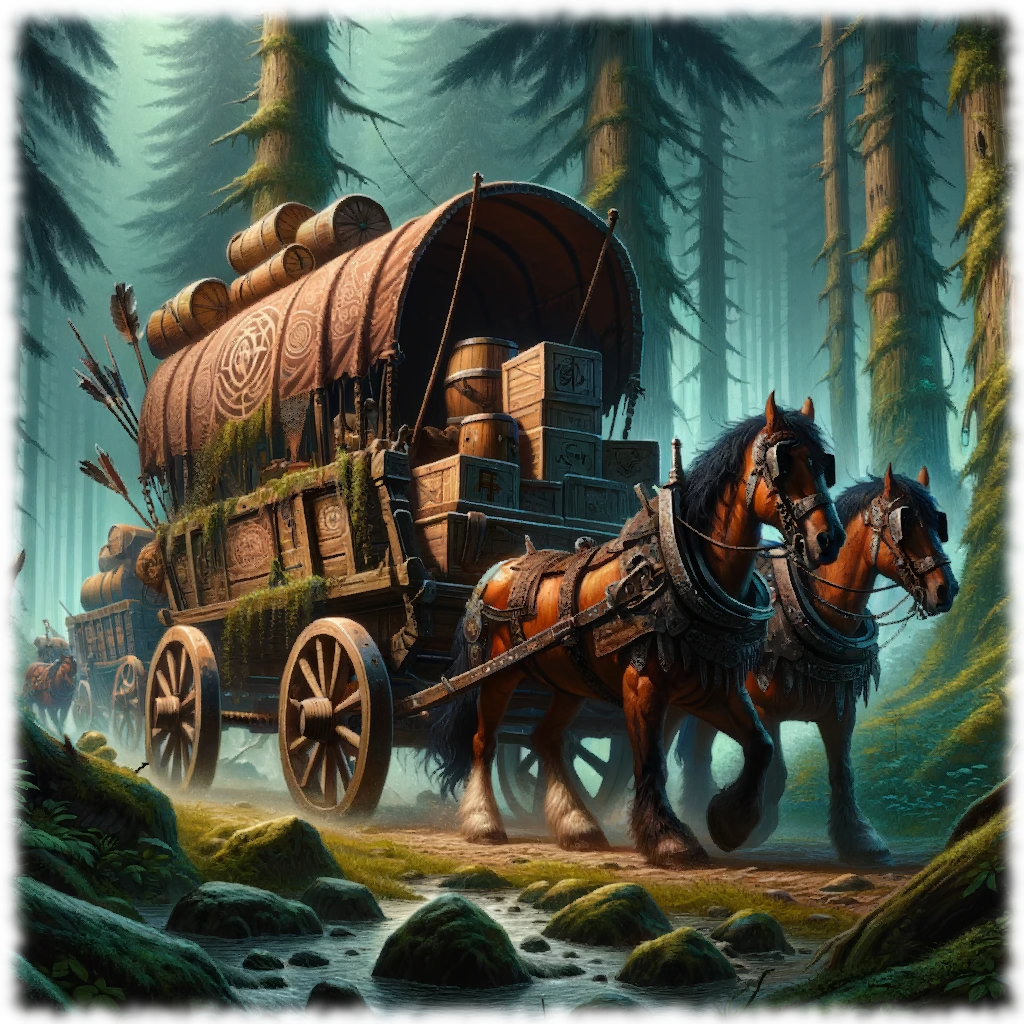
\includegraphics[scale=0.24]{img/ai-images/carriage.png}
\end{center}
\end{figure}

\section{Food \& Lodging}
Some example prices for food and lodging can be found in the following table.

\begin{table}[H]
\begin{center}
\caption{Food and Lodging}
\label{tab:food-and-lodging}
\begin{rpg-table}[|X|c|]
	\hline
	\textbf{Animal} & \textbf{Cost}\\
	\hline
	Lodging, Poor                   & 2 CP\\
	Lodging, Average                & 1 SP\\
	Lodging, Superior               & 5 SP\\
	Food and Drink, Poor, 1 Day     & 1 CP\\
	Food and Drink, Average, 1 Day  & 5 CP\\
	Food and Drink, Superior, 1 Day & 2 SP\\
	Trail Rations, 1 Day            & 5 CP\\
	\hline
\end{rpg-table}
\end{center}
\end{table}

\vspace{6em}

\begin{figure}[h]
\begin{center}

\includegraphics[scale=0.48]{img/ai-images/desert-sunset.png}
\end{center}
\end{figure}
